%
% main.tex -- Paper zum Thema <000template>
%
% (c) 2020 Hochschule Rapperswil
%
\chapter{Thema\label{chapter:000template}}
\lhead{Thema}
\begin{refsection}
\chapterauthor{Hans Muster}

Ein paar Hinweise für die korrekte Formatierung des Textes
\begin{itemize}
\item
Absätze werden gebildet, indem man eine Leerzeile einfügt.
Die Verwendung von \verb+\\+ ist nur in Tabellen und Arrays gestattet.
\item
Die explizite Platzierung von Bildern ist nicht erlaubt, entsprechende
Optionen werden gelöscht. 
Verwenden Sie Labels und Verweise, um auf Bilder hinzuweisen.
\item
Beginnen Sie jeden Satz auf einer neuen Zeile. 
Damit ermöglichen Sie dem Versionsverwaltungssysteme, Änderungen
in verschiedenen Sätzen von verschiedenen Autoren ohne Konflikt 
anzuwenden.
\item 
Bilden Sie auch für Formeln kurze Zeilen, einerseits der besseren
Übersicht wegen, aber auch um GIT die Arbeit zu erleichtern.
\end{itemize}

%
% teil1.tex -- Beispiel-File für das Paper
%
% (c) 2020 Prof Dr Andreas Müller, Hochschule Rapperswil
%
\section{Einleitung
\label{mceliece:section:einleitung}}
\rhead{Einleitung}
Beim McEliece-Kryptosystem handelt es sich um ein asymetrisches Verschlüsselungsverfahren, welches erlaubt,
Daten verschlüsselt über ein Netzwerk zu übermitteln, ohne dass vorab ein gemeinsamer,
geheimer Schlüssel unter den Teilnehmern ausgetauscht werden müsste.
Eine andere, bereits erläuterte Variante einer asymetrischen Verschlüsselung ist das Diffie-Hellman-Verfahren \ref{buch:subsection:diffie-hellman}.
Im Gegensatz zu Diffie-Hellman gilt das McEliece-System als Quantencomputerresistent
und das Verschlüsseln/Entschlüsseln von Nachrichten wird hauptsächlich mit Matrizenoperationen durchgeführt.



%
% teil1.tex -- Beispiel-File für das Paper
%
% (c) 2020 Prof Dr Andreas Müller, Hochschule Rapperswil
%
\section{Laufzeiten von Algorithmen}
\rhead{Problemstellung}
Wegen der breiten Anwendung der Matrizenmultiplikation ist eine effiziente Ausführung dieser Operation von grosser Bedeutung.
Das Ziel dieses Papers ist, verschiedenen Algorithmen der Matrizenmultiplikation vorzustellen.
Gezielt wird auf Algorithmen eingegangen, welche das Problem schneller als der Standardalgorithmus l\"osen.

\label{muliplikation:sec:bigo}
Die Big $\mathcal{O}$ Notation beschreibt die Laufzeitkomplexit\"at eines Algorithmus in Abhängigkeit zur Inputgrösse \cite{multiplikation:bigo}.
$f(x) \in \mathcal{O}(g(x))$ besagt, dass die Funktion $f$ nicht wesentlich schneller w\"achst als $g$ wenn $x \rightarrow \infty$.
Dies ist gegeben, wenn es für $f \in \mathcal{O}(n^k)$ eine Konstante $C$ gibt, mit $f(n) \leq Cn^k$.
% Es gibt eine Konstante $K$ derart, dass $f(x) \le K g(x)$ für $x\to\infty$.
Vereinfacht werden f\"ur Algorithmen die folgende Sprechweise verwendet:
\begin{itemize}
	\item $f \in \mathcal{O}(1) \rightarrow f$ ist beschr\"ankt
	\item $f \in \mathcal{O}(n) \rightarrow f$ w\"achst linear
	\item $f \in \mathcal{O}  (n^2   ) \rightarrow f$ w\"achst quadratisch
	\item $f \in \mathcal{O}(\log n) \rightarrow f$ w\"achst logarithmisch
	\item $f \in \mathcal{O}(n \log n) \rightarrow f$ hat super-lineares Wachstum
	\item $f \in \mathcal{O}  (e^n   ) \rightarrow f$ w\"achst exponentiell
	\item usw.
\end{itemize}

Konstanten werden nicht beachtet, eine Laufzeit von  $4n^2$ führt, falls $n \rightarrow \infty$ zu $\mathcal{O}(n^2)$.
In der Abbildung \ref{multiplikation:fig:bigo} k\"onnen die verschiedenen Laufzeiten miteinander verglichen werden.
Bei einer doppelt logarithmischen Darstellung werden Polynome der Form $f(x) = x^k$ als Gerade und Exponentialfunktionen der Form $f(x) = a^x$ als nach oben gekr\"ummte Kurven abgebildet.



\subsubsection{Beispiel Algorithmen}

Es folgen einige Beispiele von Algorithmen, welche zu einer bestimmten Zeitkomplexit\"atsklasse zugeteilt werden k\"onnen.


\begin{table}[t]
	\begin{tabular}{ll}
		\begin{minipage}{0.48\textwidth}
			\begin{algorithm}[H]\footnotesize\caption{}
				\label{multiplikation:alg:b1}
				\setlength{\lineskip}{7pt}
				\begin{algorithmic}
					\Function{B1}{$a, b$}
					\State \textbf{return} $a+b$
					\EndFunction
					\State
					\State
				\end{algorithmic}
			\end{algorithm}
		\end{minipage}
		&
		\begin{minipage}{0.48\textwidth}
			\begin{algorithm}[H]\footnotesize\caption{}
				\label{multiplikation:alg:b2}
				\setlength{\lineskip}{7pt}
				\begin{algorithmic}
					\Function{B2}{$a, b$}
					\State $ x \gets a+b $
					\State $ y \gets a \cdot b $
					\State \textbf{return} $x+y$
					\EndFunction
				\end{algorithmic}
			\end{algorithm}

		\end{minipage}
	\end{tabular}
\end{table}

\begin{table}
	\begin{tabular}[t]{ll}
		\begin{minipage}{0.48\textwidth}
			\begin{algorithm}[H]\footnotesize\caption{}
				\setlength{\lineskip}{7pt}
				\begin{algorithmic}
					\label{multiplikation:alg:linear}
					\Function{L}{$\mathbf{a}, \mathbf{b}$,n}
					\State $ sum \gets 0$
					\For{$i = 0,1,2 \dots,n$}
					\State $ sum \gets sum + A[i] \cdot B[i] $
					\EndFor

					\State \textbf{return} $sum$

					\EndFunction
					\State
					\State
				\end{algorithmic}
			\end{algorithm}
		\end{minipage}
		&
		\begin{minipage}{0.48\textwidth}
			\begin{algorithm}[H]\footnotesize\caption{}
				\label{multiplikation:alg:q1}
				\setlength{\lineskip}{7pt}
				\begin{algorithmic}
					\Function{Q}{$\mathbf{A}, \mathbf{B}$,n}
					\State $ sum \gets 0$
					\For{$i = 0,1,2 \dots,n$}
					\For{$j = 0,1,2 \dots,n$}
					\State $ sum \gets sum + A[i] \cdot B[j] $
					\EndFor
					\EndFor
					\State \textbf{return} $sum$
					\EndFunction
				\end{algorithmic}
			\end{algorithm}
		\end{minipage}
	\end{tabular}
\end{table}

\paragraph{Beschr\"ankter Algorithmus}
Algorithmus \ref{multiplikation:alg:b1} ist ein Beispiel mit beschränkter Laufzeit $\mathcal{O}(1)$
Da $a$ und $b$ Skalare sind, hat keine Gr\"osse $n$ einen Einfluss auf die Laufzeit.

Wie erwähnt, werden konstanten nicht beachtet, der Algorithmus \ref{multiplikation:alg:b2} f\"uhrt ebenso zu  $\mathcal{O}(1)$ und nicht zu $\mathcal{O}(2)$.


\paragraph{Linearer Algorithmus}

Der Algorithmus \ref{multiplikation:alg:linear} hat ein lineares Verhalten.
Die \texttt{for}-Schleife wird $n$-mal durchlaufen und f\"uhrt deshalb zu $\mathcal{O}(n)$.

\paragraph{Quadratischer Algorithmus}

Der Algorithmus \ref{multiplikation:alg:q1} hat ein quadratisches Verhalten.
Die beiden \texttt{for}-Schleifen werden jeweils $n$-mal durchlaufen und f\"uhrt deshalb zu $\mathcal{O} (n^2 )$.


\begin{figure}
	\center
	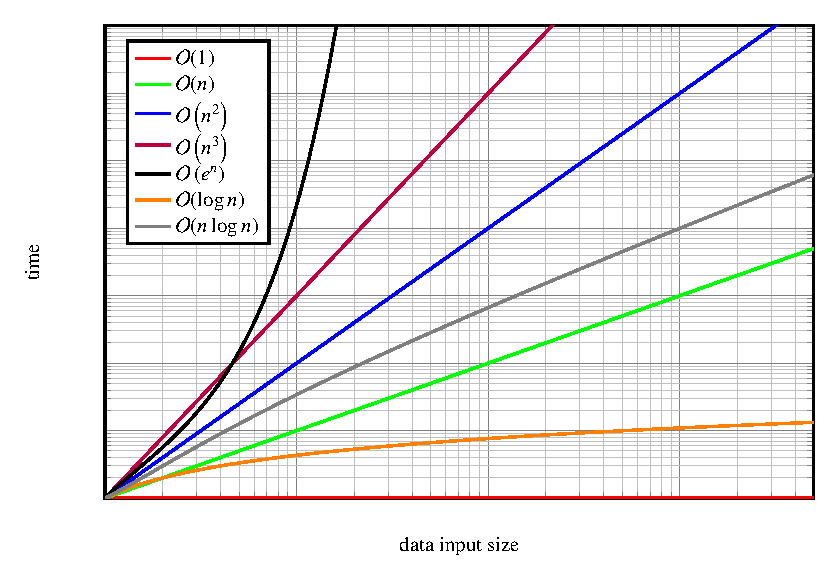
\includegraphics[]{papers/multiplikation/images/bigo}
	\caption{Laufzeiten von verschiedensten Zeitkomplexitäten. Bei einer logarithmischen Darstellung werden Polynome der Form $f(x) = x^k$ als Gerade und Exponentialfunktionen der Form $f(x) = a^x$ als nach oben gekr\"ummte Kurven dargestellt.}
	\label{multiplikation:fig:bigo}
\end{figure}

%
% loesung.tex -- Beispiel-File für die Beschreibung der Loesung
%
% (c) 2020 Prof Dr Andreas Müller, Hochschule Rapperswil
%
\section{Lösung
\label{000template:section:loesung}}
\rhead{Lösung}
Sed ut perspiciatis unde omnis iste natus error sit voluptatem
accusantium doloremque laudantium, totam rem aperiam, eaque ipsa
quae ab illo inventore veritatis et quasi architecto beatae vitae
dicta sunt explicabo. Nemo enim ipsam voluptatem quia voluptas sit
aspernatur aut odit aut fugit, sed quia consequuntur magni dolores
eos qui ratione voluptatem sequi nesciunt. Neque porro quisquam
est, qui dolorem ipsum quia dolor sit amet, consectetur, adipisci
velit, sed quia non numquam eius modi tempora incidunt ut labore
et dolore magnam aliquam quaerat voluptatem. Ut enim ad minima
veniam, quis nostrum exercitationem ullam corporis suscipit laboriosam,
nisi ut aliquid ex ea commodi consequatur? Quis autem vel eum iure
reprehenderit qui in ea voluptate velit esse quam nihil molestiae
consequatur, vel illum qui dolorem eum fugiat quo voluptas nulla
pariatur?

\subsection{De finibus bonorum et malorum
\label{000template:subsection:bonorum}}
At vero eos et accusamus et iusto odio dignissimos ducimus qui
blanditiis praesentium voluptatum deleniti atque corrupti quos
dolores et quas molestias excepturi sint occaecati cupiditate non
provident, similique sunt in culpa qui officia deserunt mollitia
animi, id est laborum et dolorum fuga. Et harum quidem rerum facilis
est et expedita distinctio. Nam libero tempore, cum soluta nobis
est eligendi optio cumque nihil impedit quo minus id quod maxime
placeat facere possimus, omnis voluptas assumenda est, omnis dolor
repellendus. Temporibus autem quibusdam et aut officiis debitis aut
rerum necessitatibus saepe eveniet ut et voluptates repudiandae
sint et molestiae non recusandae. Itaque earum rerum hic tenetur a
sapiente delectus, ut aut reiciendis voluptatibus maiores alias
consequatur aut perferendis doloribus asperiores repellat.



%
% problemstellung.tex -- Beispiel-File für die Beschreibung des Problems
%
% (c) 2020 Prof Dr Andreas Müller, Hochschule Rapperswil
%
\section{Folgerungen
\label{000template:section:folgerungen}}
\rhead{Folgerungen}
Sed ut perspiciatis unde omnis iste natus error sit voluptatem
accusantium doloremque laudantium, totam rem aperiam, eaque ipsa
quae ab illo inventore veritatis et quasi architecto beatae vitae
dicta sunt explicabo. Nemo enim ipsam voluptatem quia voluptas sit
aspernatur aut odit aut fugit, sed quia consequuntur magni dolores
eos qui ratione voluptatem sequi nesciunt. Neque porro quisquam
est, qui dolorem ipsum quia dolor sit amet, consectetur, adipisci
velit, sed quia non numquam eius modi tempora incidunt ut labore
et dolore magnam aliquam quaerat voluptatem. Ut enim ad minima
veniam, quis nostrum exercitationem ullam corporis suscipit laboriosam,
nisi ut aliquid ex ea commodi consequatur? Quis autem vel eum iure
reprehenderit qui in ea voluptate velit esse quam nihil molestiae
consequatur, vel illum qui dolorem eum fugiat quo voluptas nulla
pariatur?

\subsection{De finibus bonorum et malorum
\label{000template:subsection:malorum}}
At vero eos et accusamus et iusto odio dignissimos ducimus qui
blanditiis praesentium voluptatum deleniti atque corrupti quos
dolores et quas molestias excepturi sint occaecati cupiditate non
provident, similique sunt in culpa qui officia deserunt mollitia
animi, id est laborum et dolorum fuga. Et harum quidem rerum facilis
est et expedita distinctio. Nam libero tempore, cum soluta nobis
est eligendi optio cumque nihil impedit quo minus id quod maxime
placeat facere possimus, omnis voluptas assumenda est, omnis dolor
repellendus. Temporibus autem quibusdam et aut officiis debitis aut
rerum necessitatibus saepe eveniet ut et voluptates repudiandae
sint et molestiae non recusandae. Itaque earum rerum hic tenetur a
sapiente delectus, ut aut reiciendis voluptatibus maiores alias
consequatur aut perferendis doloribus asperiores repellat.




\printbibliography[heading=subbibliography]
\end{refsection}
